\documentclass{standalone}
\usepackage{tikz}
\usepackage{bm}
\usetikzlibrary{decorations.pathmorphing, patterns, arrows, decorations.markings}
\begin{document}
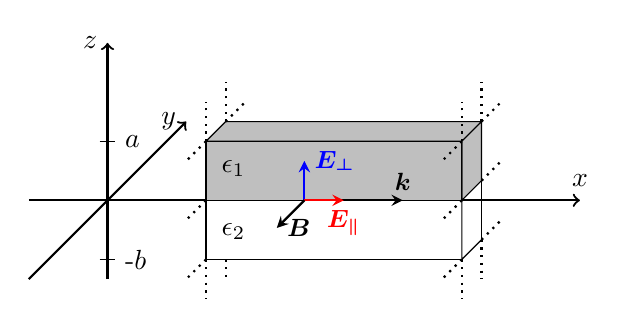
\begin{tikzpicture}
    %\draw [help lines, step=0.5cm] (-2.5,-2.5) grid (6,3);
    
    % Axes
    \draw[->, thick] (-1,0)  -- (6,0,0);
    \node at (6,0.25) {$x$};
    
    \draw[->, thick] (-1,-1) -- (1,1) node[left] {$y$};
    \draw[->, thick] (0,-1) -- (0,2) node[left] {$z$};
    
    \node (T1) at (1.25,0.75) {};
    \node (T2) at (1.5,1) {};
    \node (T3) at (4.5,0.75) {};
    \node (T4) at (4.75,1) {};
    
    \node (B1) at (1.25,-0.75) {};
    \node (B2) at (4.5,-0.75) {};
    \node (B3) at (4.75,-0.5) {};
    
    % Stratification
    %\node at (-0.2,1.2) {$a$};
    \draw[fill=gray!50] (T1.center) -- (T3.center) -- (T4.center) -- (T2.center) -- (T1.center);

    %\node at (-0.2,-0.8) {-$b$};
    \draw (B1.center) -- (B2.center);
    \draw (T1) -- (T2);
    
    \draw[fill=gray!50] (1.25,0) -- (T1.center) -- (T3.center) -- (4.5,0) -- (1.25,0);
    \draw[fill=gray!50] (4.5,0) -- (4.5,0.75) -- (T4.center) -- (4.75,0.25) -- (4.5,0);
    
    \draw (T1.center) -- (B1.center);
    \draw (T3.center) -- (B2.center)  -- (B3.center);
    \draw (T4.center) -- (B3.center);
    
    % Dotted lines
    \draw[dotted, thick] (B1.center) -- (1,-1);
    \draw[dotted, thick] (B1.center) -- (1.25,-1.25);
    \draw[dotted, thick] (T1.center) -- (1,0.5);
    \draw[dotted, thick] (T1.center) -- (1.25,1.25);
    \draw[dotted, thick] (T2.center) -- (1.5,1.5);
    \draw[dotted, thick] (1.25,0) -- (1,-0.25);
    \draw[dotted, thick] (T2.center) -- (1.75,1.25);
    
    \draw[dotted, thick] (B2.center) -- (4.25,-1);
    \draw[dotted, thick] (4.5,0) -- (4.25,-0.25);
    \draw[dotted, thick] (4.5,0.75) -- (4.25,0.5);
    \draw[dotted, thick] (B2.center) -- (4.5,-1.25);
    \draw[dotted, thick] (B3.center) -- (4.75,-1);
    \draw[dotted, thick] (B3.center) -- (5,-0.25);
    \draw[dotted, thick] (4.75, 0.25) -- (5,0.5);
    \draw[dotted, thick] (T4.center) -- (5,1.25);
    
    \draw[dotted, thick] (T3.center) -- (4.5,1.25);
    \draw[dotted, thick] (T4.center) -- (4.75,1.5);
    \draw[dotted, thick] (1.5,-0.75) -- (1.5,-1);
    
    % Field arrows
    \draw[->, thick, >=stealth] (2.5,0) -- (3.75,0) node[above] {\small $\bm{k}$};
    \draw[->, thick, >=stealth, blue] (2.5,0) -- (2.5,0.5) node[right] {\small $\bm{E_{\bot}}$};
    \draw[->, thick, >=stealth, red] (2.5,0) -- (3,0) node[below] {\small $\bm{E_{\parallel}}$};
    \draw[->, thick, >=stealth] (2.5,0) -- (2.15,-0.35) node[right] {\small $\bm{B}$};
    
    % labels
    \node at (1.6,0.4) {$\epsilon_1$};
    \node at (1.6,-0.4) {$\epsilon_2$};
    \draw (-0.1,-0.75) -- (0.1,-0.75) node[right] {-$b$};
    \draw (-0.1,0.75) -- (0.1,0.75) node[right] {$a$};
    %\node at (1.85,1.23) {\footnotesize $\bm{E_{\bot}}$};
    %\node at (0.675,0.825) {\footnotesize $\bm{E_{\parallel}}$};
    
\end{tikzpicture}
\end{document}